\section{Motivation}
% \note{jk: Give context about Lucene and page cache and then say how TeraHeap is
% used to offload cached data over the storage device. Then say that we evaluate
% how page cache and heap size accordingly affects execution.}

\note{Start the section showing the purpose.. what is your purpose for the
motivation.. what is your goal? what are you trying to show.. Then explain why
you select Lucene as a usecase.} 

\note{rewrite the motivation because it is like reading the intro again!!!
Another option is to merge it with intro... Think about it!}

Lucene is a widely used full-text search engine library that powers indexing and
querying for large-scale data analytics and enterprise search applications. To
deliver low-latency query responses, Lucene relies heavily on managed heap
memory to store its indexing structures, query evaluation data and internal
caches. In particular, the page cache plays a crucial role by caching index
segments and frequently accessed postings lists, reducing I/O latency during
searches. However, as datasets grow, DRAM capacity becomes insufficient to hold
all required data and caches.

\note{remove this paragraph... you write the same thing in intro... }
To overcome these limitations, TeraHeap extends the JVM managed heap beyond DRAM capacity by partitioning 
it into two regions: a primary heap (H1) in DRAM for GC-managed short-lived objects and a secondary heap 
(H2) mapped to fast NVMe SSD storage for longer-lived cached data such as Lucene’s query cache. This hybrid 
design allows TeraHeap to confine garbage collection activity to H1, avoiding expensive GC scans over large
cached data stored in H2, while using DRAM both for heap allocations and as a page cache to accelerate H2 accesses.

\note{again!! you write the same thing in intro... read the text carefully and
remove duplicate things.}
However, TeraHeap statically divides DRAM between H1 and the page cache for H2 at JVM launch time, introducing 
significant performance limitations. If H1 is too small, Lucene experiences high GC overhead due to frequent collections, 
negatively impacting indexing and query latency. Conversely, if the DRAM page cache for H2 is too small, accessing Lucene’s 
index segments stored in H2 incurs high I/O latency, degrading search throughput. Because Lucene workloads exhibit varying 
memory demands such as bulk indexing phases require large heaps to minimize GC, while read-heavy query workloads benefit 
from a larger page cache static DRAM partitioning fails to adapt to these changing phases, resulting in suboptimal performance.

In this work, we evaluate how dynamically adjusting the division of DRAM between H1 and the page cache in TeraHeap affects Lucene 
performance under DRAM constraints. By resizing H1 at runtime based on GC and I/O costs, our approach aims to maintain low GC overhead
during memory-intensive phases while ensuring sufficient page cache capacity to accelerate I/O-heavy query workloads, ultimately improving
end-to-end performance.

The figure \ref{fig:graph} illustrates the breakdown of Lucene’s total execution
time into GC time and non-GC (other) time under different page cache
configurations. The x-axis represents the fraction of DRAM allocated to the page
cache (10\%, 20\%, 30\%, 40\%, etc.), while the y-axis shows the average total
execution time in seconds for each configuration.

\begin{figure}[htbp]
  \centering
  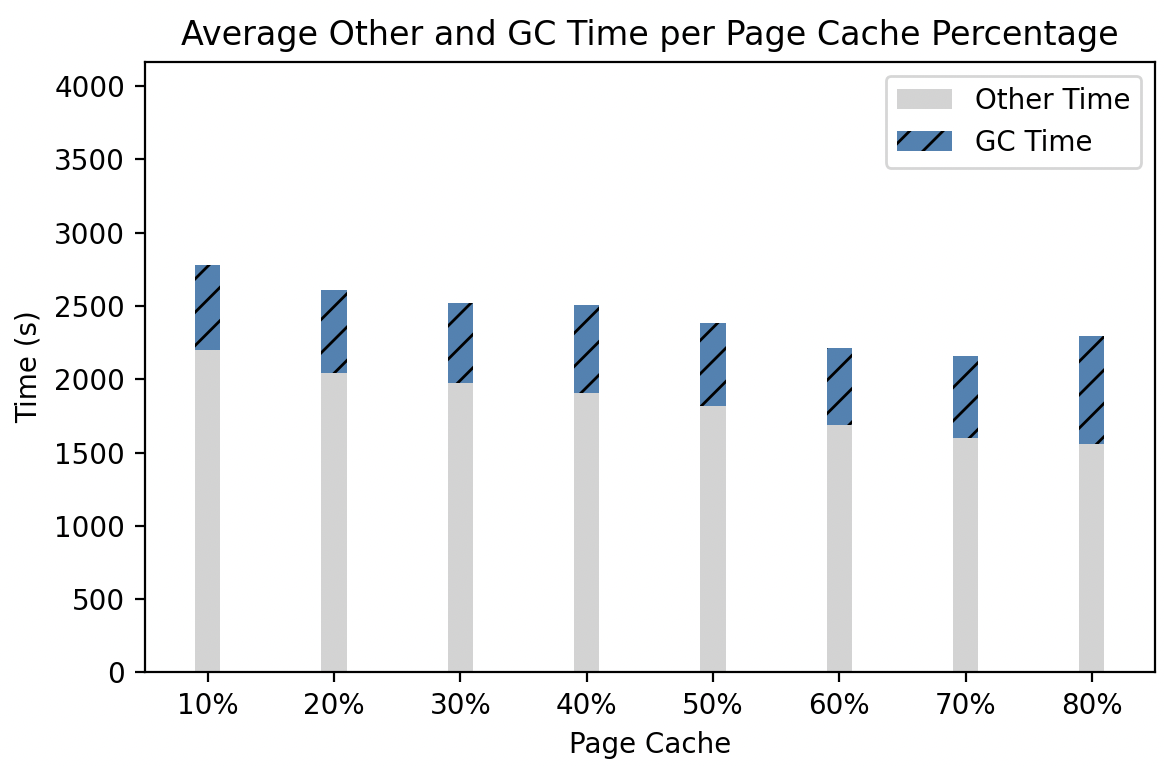
\includegraphics[width=1\columnwidth]{fig/numbers.png}
  \caption{Graph of different H1/page cache configurations}
  \label{fig:graph}
\end{figure}

At low page cache allocations (10\% to 30\%), the GC time is minimal relative to total execution time. However, as the page cache share grows (40\% to 60\%), GC time steadily increases. This is because increasing page cache size reduces the available DRAM allocated to H1, resulting in a smaller primary heap. A smaller heap triggers more frequent garbage collections, leading to higher GC overhead.
The grey part of each bar represents the time spent executing Lucene and system operations excluding GC. As the page cache share increases, the non-GC time decreases. This is because a larger page cache reduces I/O latency when accessing index segments stored in H2 (SSD) such as Lucene's query cache.
The graph captures the tradeoff in TeraHeap’s static DRAM partitioning: \vspace{-0.5em} 
\begin{itemize} 
  \item Allocating more DRAM to H1 results in a larger heap, reducing GC time but yielding a smaller page cache, which increases I/O latency and non-GC execution time.
  \item Allocating more DRAM to the page cache reduces I/O latency and non-GC execution time but increases GC overhead due to the smaller H1.
\end{itemize} 
\vspace{-0.5em}

I/O Wait Analysis. Figure~\ref{fig:iowait} illustrates the I/O wait percentage over time during the execution of a Lucene workload. We observe that 
I/O wait exhibits significant variability, with spikes reaching above 20\% but generally remaining under 10\% for most of the 
execution. This variability indicates that the I/O demand of the workload is highly dynamic, between phases of low and high storage access 
intensity. Such behavior underscores the limitations of static DRAM configurations,
which cannot adapt to changing workload phases. 


\begin{figure}[htbp]
  \centering
  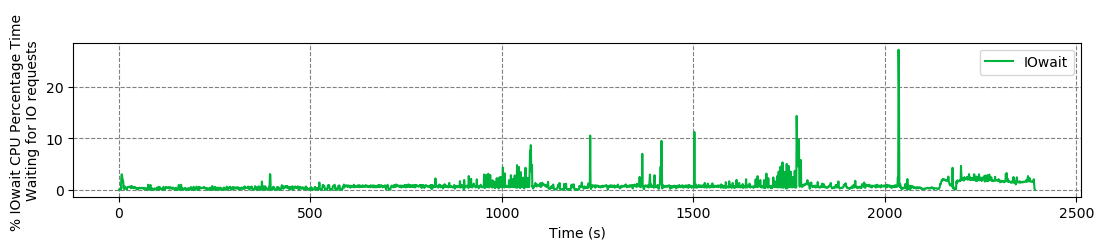
\includegraphics[width=1\columnwidth]{fig/iow_cpu.png}
  \caption{Graph of iowait during the execution of a lucene benchmark with 20GB H1 and 20GB H2 page cache}
  \label{fig:iowait}
\end{figure}

Both graphs indicate that there is potential for optimization by introducing a dynamic heap resizer that adjusts the H1 size at runtime based on workload phases and memory pressure. Such an approach could balance the trade-offs between configurations by reducing GC time during indexing while also minimizing I/O latency during query processing. 
